\documentclass[conference]{IEEEtran}
\IEEEoverridecommandlockouts
% The preceding line is only needed to identify funding in the first footnote. If that is unneeded, please comment it out.
\usepackage{cite}
\usepackage{amsmath,amssymb,amsfonts}
\usepackage{algorithmic}
\usepackage{graphicx}
\usepackage{textcomp}
\usepackage{xcolor}
\usepackage{listings}                           %顯示code用的
\usepackage{fontspec}                           %設定字體
\usepackage[CheckSingle, CJKmath]{xeCJK}
\usepackage{CJKulem}
\usepackage{listings}
\usepackage{color} %red, green, blue, yellow, cyan, magenta, black, white
\usepackage{float}

\definecolor{mygreen}{RGB}{28,172,0} % color values Red, Green, Blue
\definecolor{mylilas}{RGB}{170,55,241}

\setmainfont{Consolas}
%\setmonofont{Ubuntu Mono}
\setmonofont{Consolas}
\setCJKmainfont{Noto Sans CJK TC}
\XeTeXlinebreaklocale "zh"                      %中文自動換行

\lstset{language=Matlab,%
    %basicstyle=\color{red},
    breaklines=true,%
    morekeywords={matlab2tikz},
    keywordstyle=\color{blue},%
    morekeywords=[2]{1}, keywordstyle=[2]{\color{black}},
    identifierstyle=\color{black},%
    stringstyle=\color{mylilas},
    commentstyle=\color{mygreen},%
    showstringspaces=false,%without this there will be a symbol in the places where there is a space
    numbers=left,%
    numberstyle={\tiny \color{black}},% size of the numbers
    numbersep=9pt, % this defines how far the numbers are from the text
    emph=[1]{for,end,break},emphstyle=[1]\color{red}, %some words to emphasise
    %emph=[2]{word1,word2}, emphstyle=[2]{style},    
}

\def\BibTeX{{\rm B\kern-.05em{\sc i\kern-.025em b}\kern-.08em
    T\kern-.1667em\lower.7ex\hbox{E}\kern-.125emX}}

\begin{document}
\title{Performace on differnet parameter setting in GA-BPNN\\
% {\footnotesize \textsuperscript{*}Note: Sub-titles are not captured in Xplore and should not be used}
% \thanks{Identify applicable funding agency here. If none, delete this.}
}

\author{\IEEEauthorblockN{1\textsuperscript{st} Zih Jie Lin}
\IEEEauthorblockA{\textit{Computer Science Information Engineering.} \\
\textit{Fu Jen Catholoic University}\\
New Taipei City, Taiwan \\
406261597@gapp.fju.edu.tw}
}
% \and
% \IEEEauthorblockN{2\textsuperscript{nd} Given Name Surname}
% \IEEEauthorblockA{\textit{dept. name of organization (of Aff.)} \\
% \textit{name of organization (of Aff.)}\\
% City, Country \\
% email address or ORCID}
% \and
% \IEEEauthorblockN{3\textsuperscript{rd} Given Name Surname}
% \IEEEauthorblockA{\textit{dept. name of organization (of Aff.)} \\
% \textit{name of organization (of Aff.)}\\
% City, Country \\
% email address or ORCID}
% \and
% \IEEEauthorblockN{4\textsuperscript{th} Given Name Surname}
% \IEEEauthorblockA{\textit{dept. name of organization (of Aff.)} \\
% \textit{name of organization (of Aff.)}\\
% City, Country \\
% email address or ORCID}
% \and
% \IEEEauthorblockN{5\textsuperscript{th} Given Name Surname}
% \IEEEauthorblockA{\textit{dept. name of organization (of Aff.)} \\
% \textit{name of organization (of Aff.)}\\
% City, Country \\
% email address or ORCID}
% \and
% \IEEEauthorblockN{6\textsuperscript{th} Given Name Surname}
% \IEEEauthorblockA{\textit{dept. name of organization (of Aff.)} \\
% \textit{name of organization (of Aff.)}\\
% City, Country \\
% email address or ORCID}

\maketitle

% \begin{abstract}
% \end{abstract}

% \begin{IEEEkeywords}
% \end{IEEEkeywords}

\section{問題一}
程式碼:\\
\lstinputlisting{problem1.m}
\begin{figure}[H]
\centerline{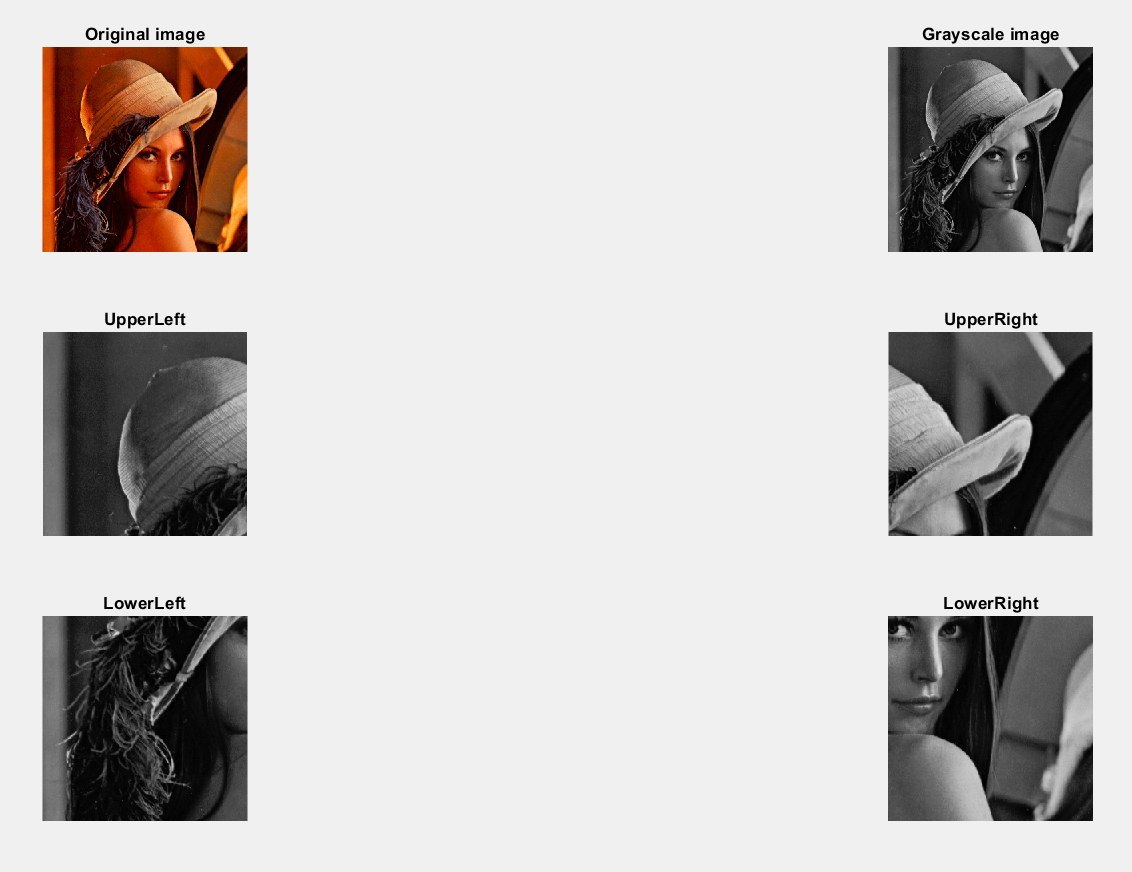
\includegraphics[width=8cm]{problem1.png}}
\caption{The result of problem1}
\label{fig}
\end{figure}

\section{問題二}
\subsection{選定辦法}
\begin{itemize}
\item Nearest-neighbor interpolation
\item Bilinear interpolation
\item Bicubic interpolation
\end{itemize}

\subsection{圖片}
\begin{figure}[H]
\centerline{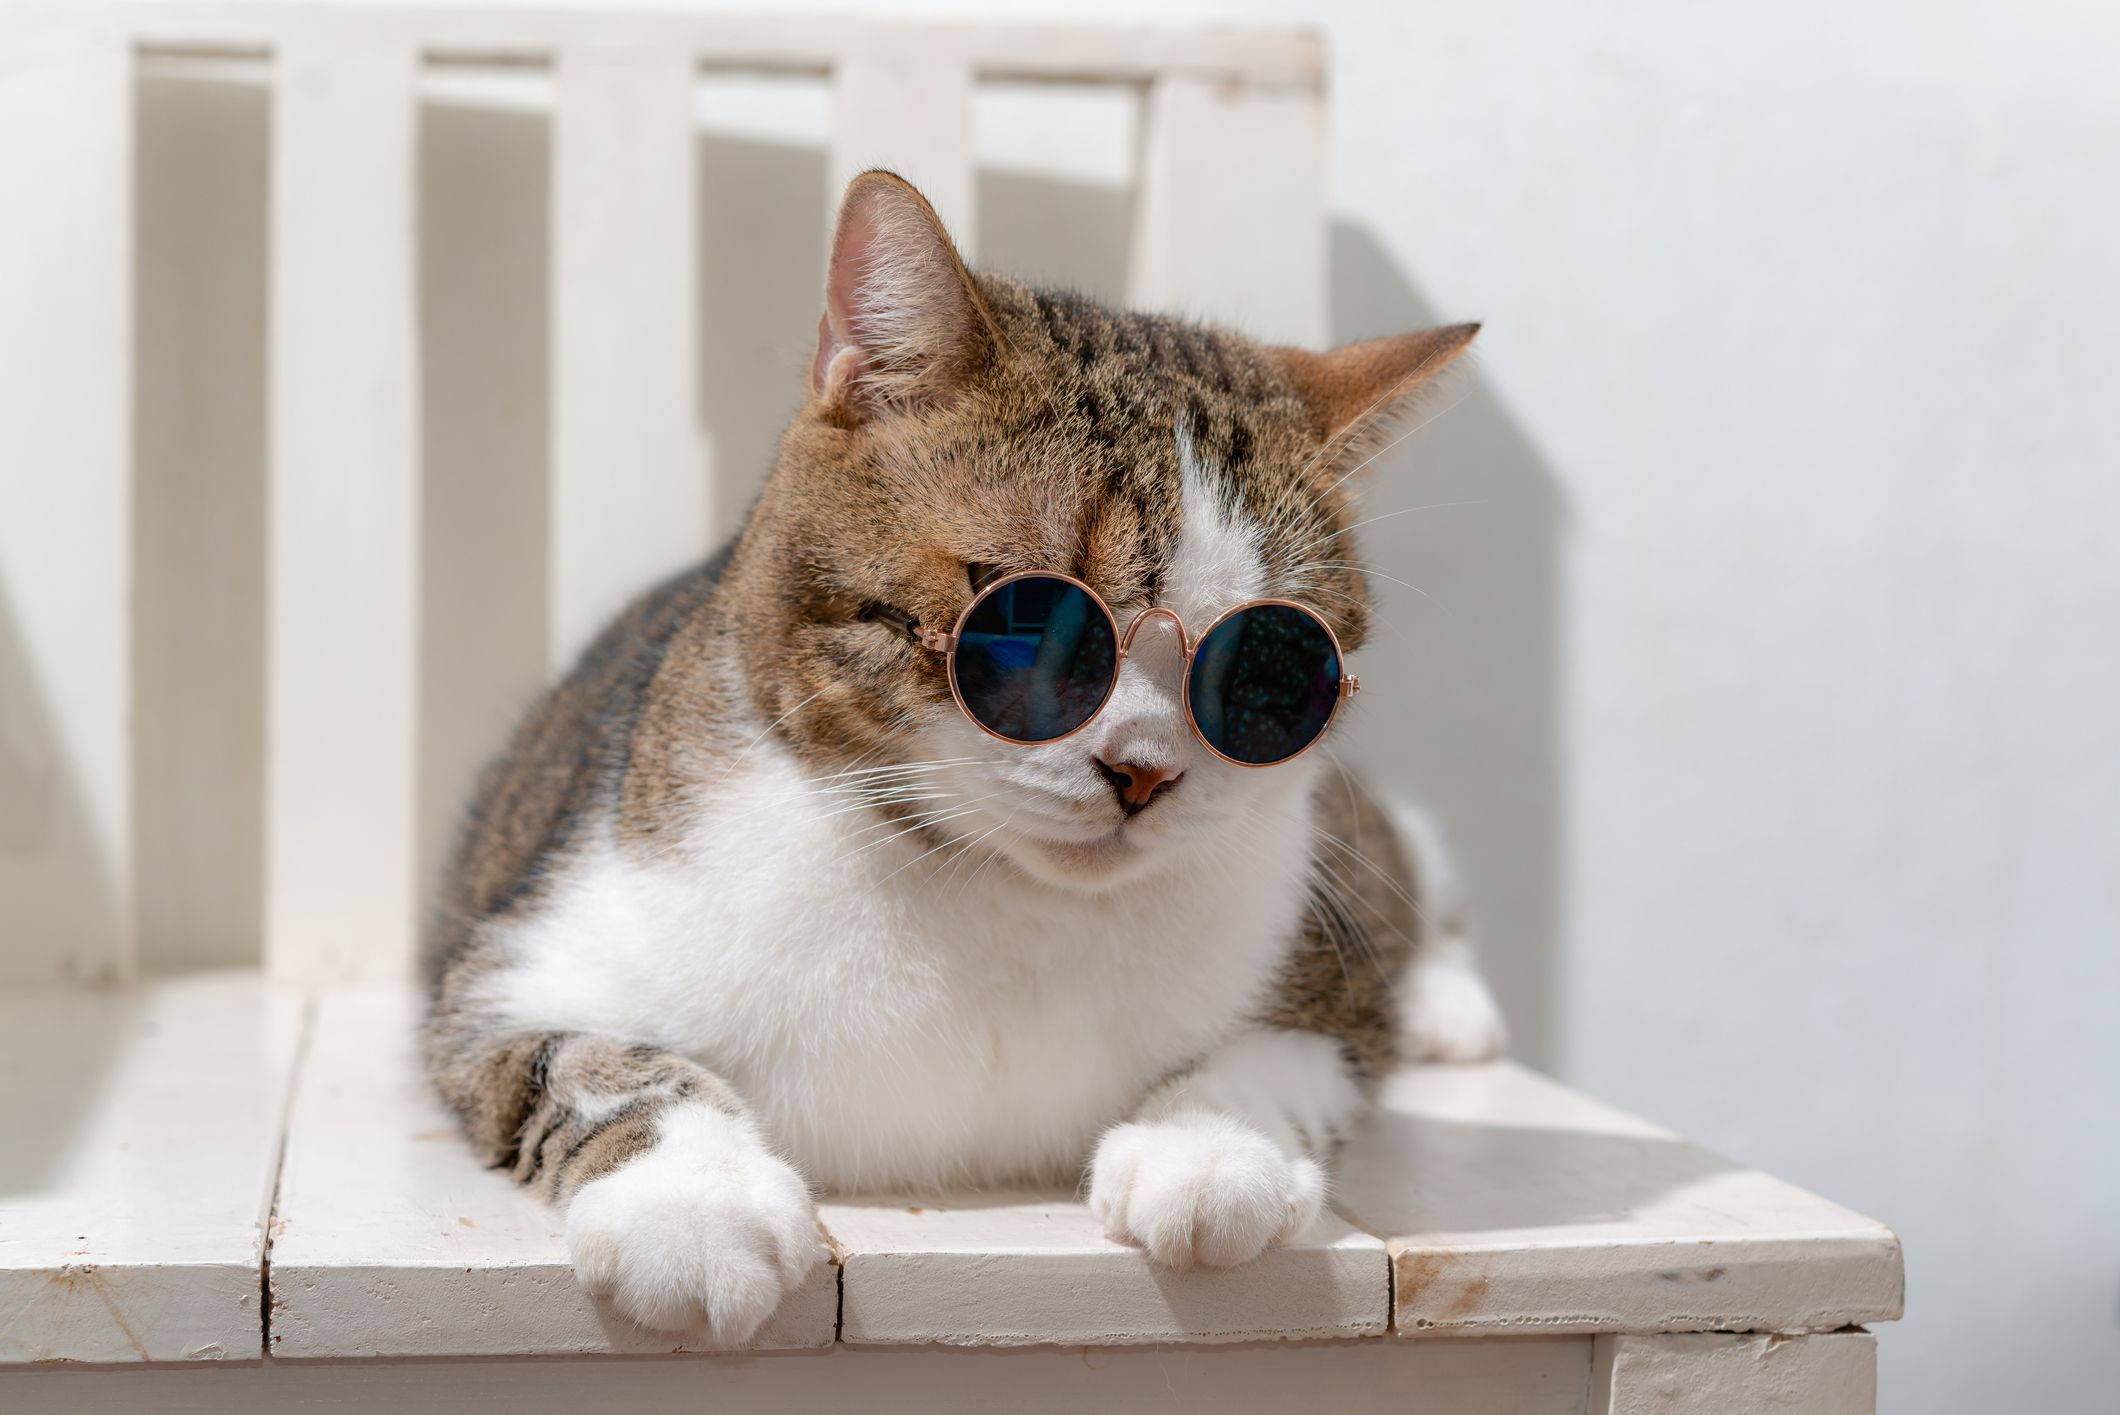
\includegraphics[width=8cm]{cat.jpg}}
\caption{Cat}
\label{fig}
\end{figure}
\begin{figure}[H]
\centerline{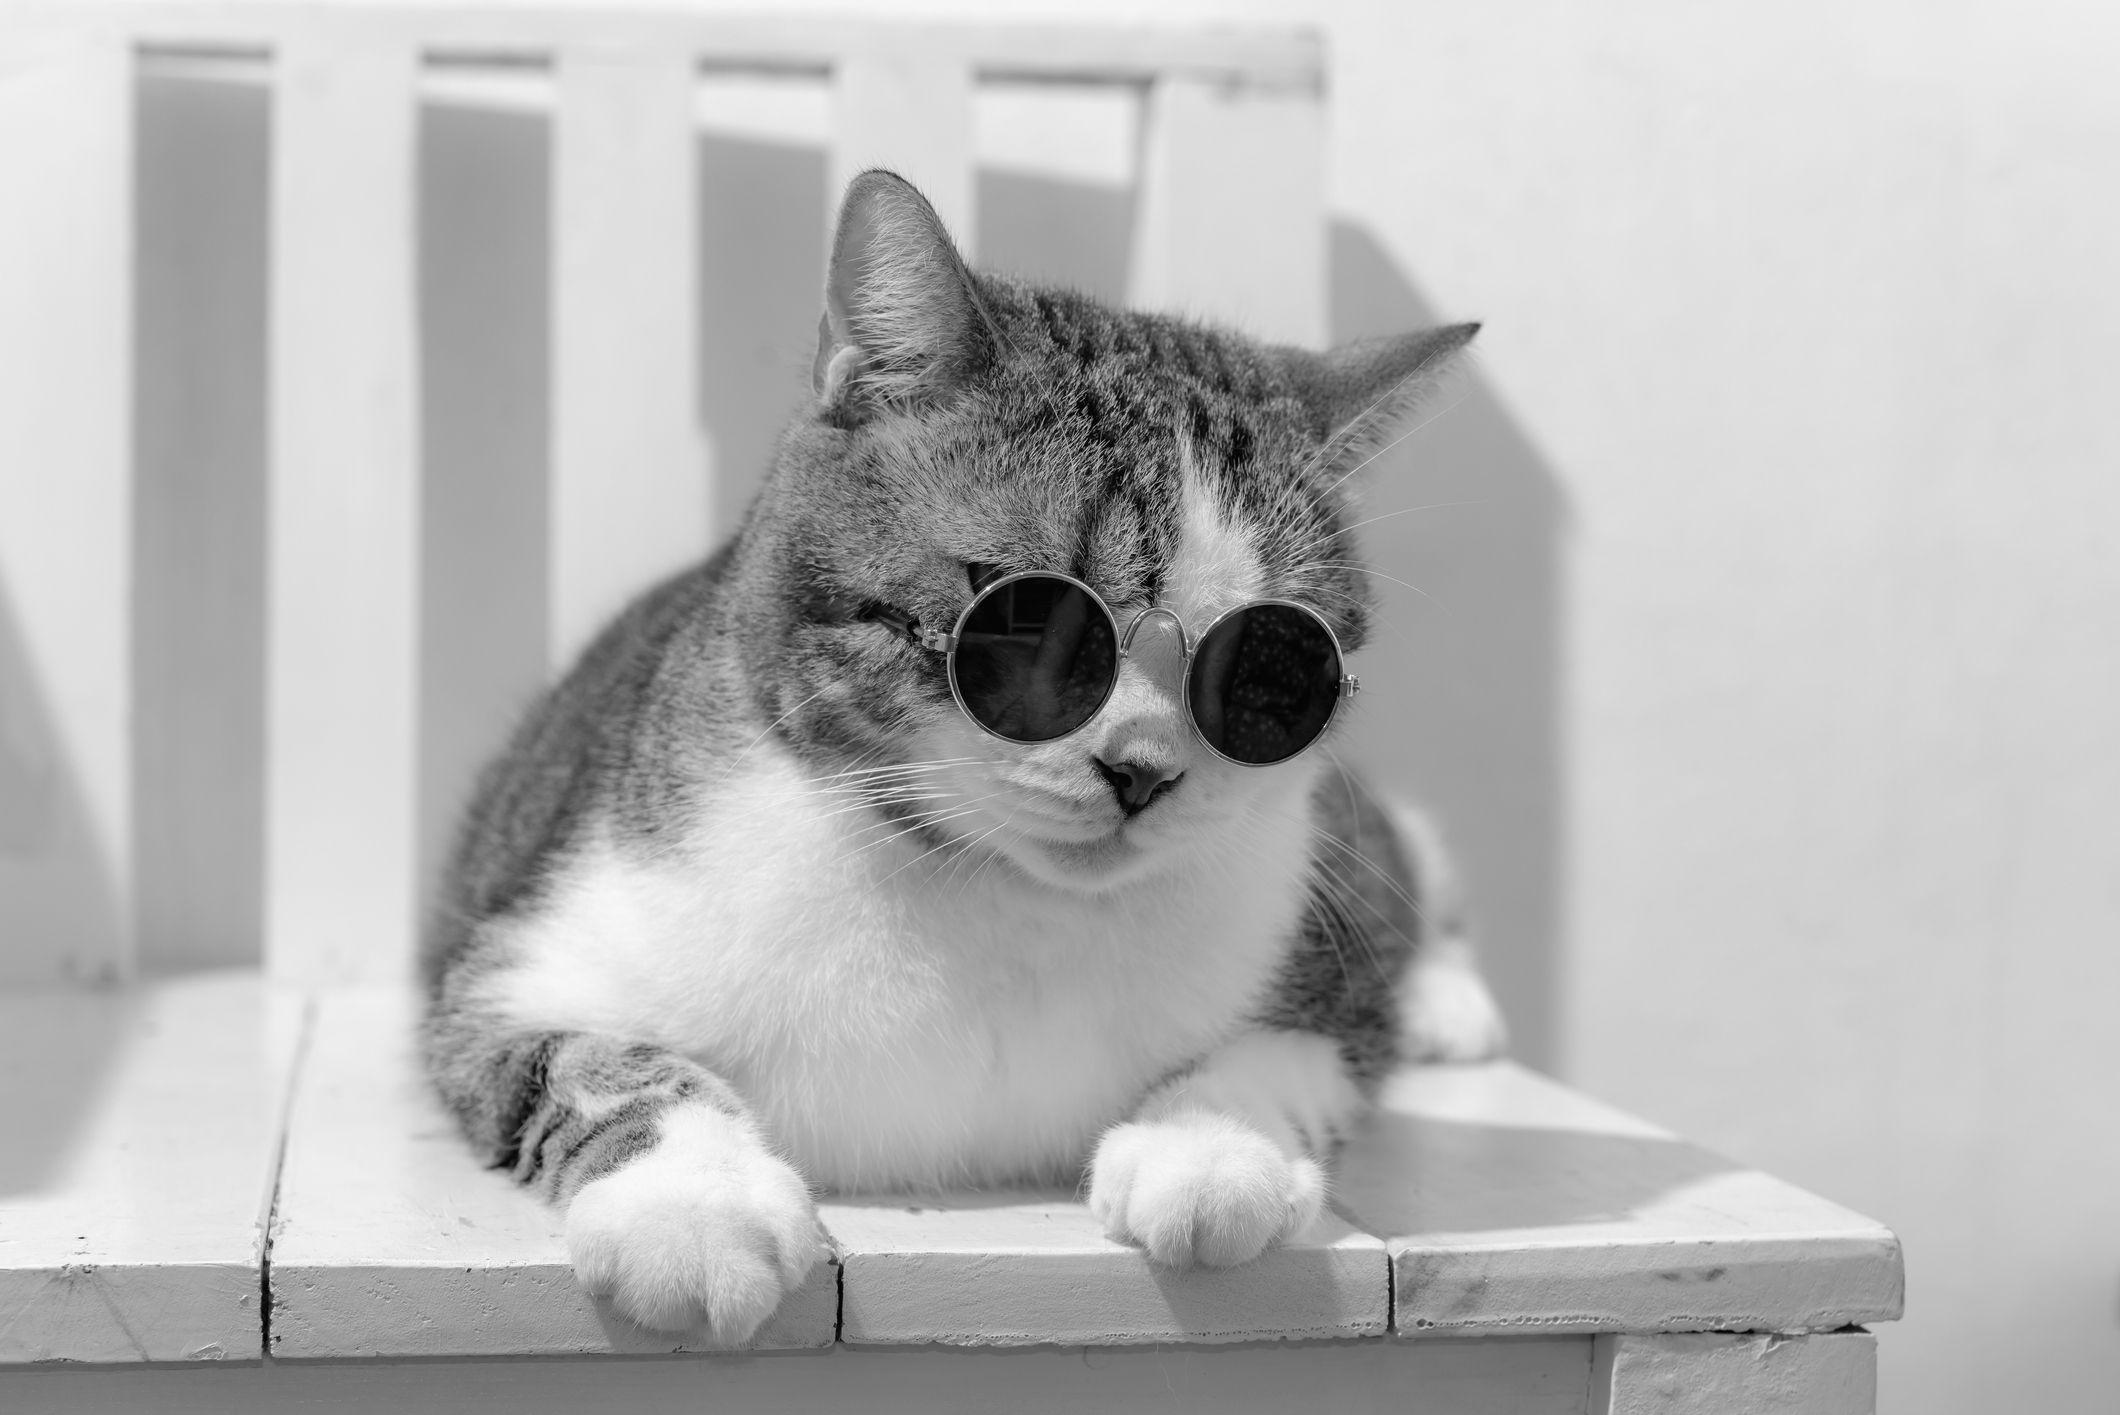
\includegraphics[width=8cm]{grayCat.jpg}}
\caption{Cat after converting to grayscale}
\label{fig}
\end{figure}

\subsection{程式碼}
\lstinputlisting{problem2.m}

\subsection{比較}
三種辦法都在縮小 7 次在復原後無法辨識為一隻貓,Nearest-neighbor interpolation 的顏色和原圖較相近。\\

隨著縮小次數增加,Nearest-neighbor interpolation 會變成一格格大黑/白點。Bilinear interpolation 則像是起霧一般,變成一小點黑白點。Bicubic interpolation 則是皆於兩者之間。

\begin{figure}[H]
\centerline{
\includegraphics[width=8cm]{grayCat1_7.jpg}}
\caption{Using Nearest-neighbor interpolation shrink the size of the image by two 7 times and undo.}
\label{fig}
\end{figure}
\begin{figure}[H]
\centerline{
\includegraphics[width=8cm]{grayCat2_7.jpg}}
\caption{Using Bilinear interpolation shrink the size of the image by two 7 times and undo.}
\label{fig}
\end{figure}
\begin{figure}[H]
\centerline{
\includegraphics[width=8cm]{grayCat3_7.jpg}}
\caption{Using Bicubic interpolation shrink the size of the image by two 7 times and undo.}
\label{fig}
\end{figure}


% \begin{thebibliography}{00}
% \end{thebibliography}

\vspace{12pt}

\end{document}
